\begin{figure}%[!b]
  \vspace{-.1cm}
\center
%% \iffalse
%% \begin{tabular}{cc}
%% \raisebox{4.6cm}{\panel{A}} & \hspace{-1cm}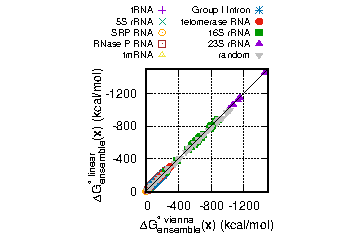
\includegraphics[width=0.3\textwidth]{figs/ensemble_xy} \\
%% % \raisebox{3.6cm}{\panel{B}}
%% \hspace{-1cm}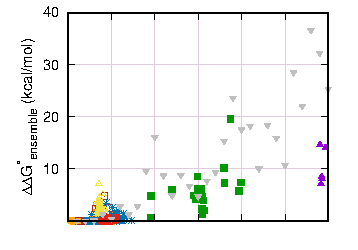
\includegraphics[width=0.2\textwidth]{figs/ensemble_len}
%%  & \hspace{-1cm}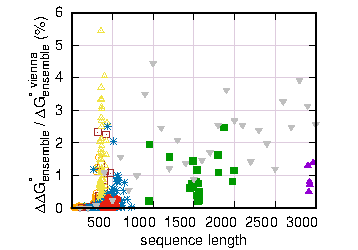
\includegraphics[width=0.2\textwidth]{figs/ensemble_len_norm} \\[-0.3cm]
%% \end{tabular}
%% \fi
%% \iffalse
%% \begin{tabular}{ccc}
%% {\panel{A}} & {\panel{B}} & {\panel{C}} \\
%% \hspace{-1cm}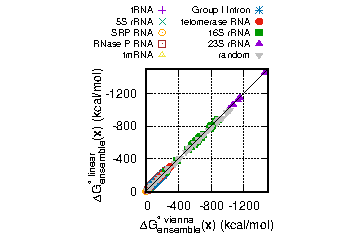
\includegraphics[width=0.3\textwidth]{figs/ensemble_xy} &
%% \hspace{-.8cm}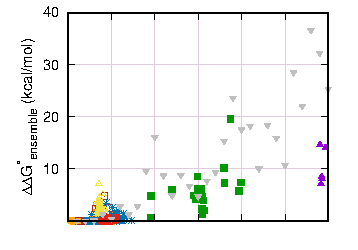
\includegraphics[width=0.3\textwidth]{figs/ensemble_len} &
%% \hspace{-.8cm}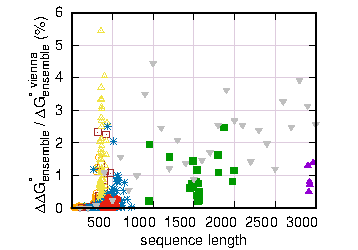
\includegraphics[width=0.3\textwidth]{figs/ensemble_len_norm} \\[-0.3cm]
%% \end{tabular}
%% \fi
\begin{tabular}{cc}
% {\panel{A}} & {\panel{B}}\\
\hspace{-0.2cm}\raisebox{2.9cm}{\panel{A}\hspace{-2.2cm}}\raisebox{2.5cm}{\multirow{2}{*}{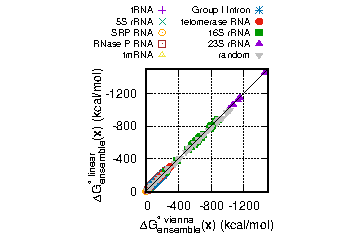
\includegraphics[width=0.47\textwidth]{figs/ensemble_xy}}} & 
\hspace{-2.4cm}\raisebox{2.9cm}{\panel{B}}\hspace{-.35cm}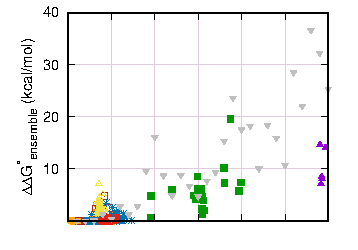
\includegraphics[scale=0.74]{figs/ensemble_len} \\[-.5cm]
% &{\panel{A}}\\
&\hspace{-2.4cm}\raisebox{2.6cm}{\panel{\color{white}C}}\hspace{-.3cm}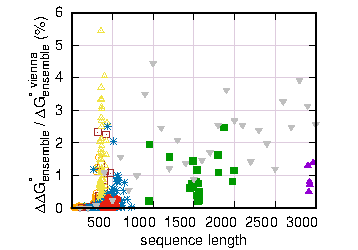
\includegraphics[scale=0.79]{figs/ensemble_len_norm} \\[-0.4cm]
\end{tabular}
\caption{
  Approximation quality of partition function  on ArchiveII dataset and random sequences. %. shorter than 3,000~\nts.
  {\bf A}: The x and y axes are
  ensemble folding free energy changes $\ensenergy(\vecx)$ of \viennarnafold %($-RT\log Q_\vienna(\vecx)$)
  and \linearpartition, % ($-RT\log Q_\linear(\vecx)$),
  respectively.
  {\bf B}: 
  Difference of ensemble folding free energy change (top), ${\ddg(\vecx)}$, between \rnafold and \linearpartition.
  and the relative differences (bottom),  ${\ddg(\vecx)}/{\ensenergyvienna(\vecx)}$, in percentages.
  %% of 
  %% ensemble folding free energy changes,
%  $\frac{ \ensenergyvienna(\vecx) - \ensenergylinear(\vecx)}{\ensenergylinear(\vecx)}$.
  \label{fig:partition}
  \vspace{-0.2cm}
}
\end{figure}
